\subsection{Robôs cabeados}
% 1 OQ SAO, MODTIVACAO
% 2 TECNOLOGIA DE FIXACAO
% 3 NOSSOS ROBOS
% Vantagens e desvantagens
%TODO características gerais do robo: fixação,
% sensores, sistema HVOF e etc
% aplicação,
% vantagens e desvantagens

São classificados como robôs cabeados quaisquer sistemas robôticos que façam
uso de um conjunto de cabos e/ou cordas para auxiliar ou mesmo garantir seu
posicionamento adequado na sua região de trabalho. Sendo assim, robôs cabeados
podem possuir outros métodos de fixação em conjunto com seu cabeamento.

A idéia do uso de um sistema de cabos surge naturalmente, quando o deslocamento
se mostra majoriamente restrito a um plano vertical e não há exigência de
grandes velocidades de deslocamento, como forma de reduzir o preso e melhorar o
desempenho de um braço mecânico de mesmo alcance, ou diminuir a complexidade e
a força de aderência necessária para um \textit{crawler}.

Para exemplificar essa categoria foram selecionados dois robôs. O
\textit{torboMate} é um \textit{crawler} que possui adesão magnética que o
permite caminhar livremente sobre toda a superfice de aço. Pode ter dois ou um
emissor de jatos (com capacidade para abastecimento em até 4000 bar). Pesa 45kg
e atinge uma velocidade de até 20 m/min \citep{torbo}.

\begin{figure}[ht]
	\centering
	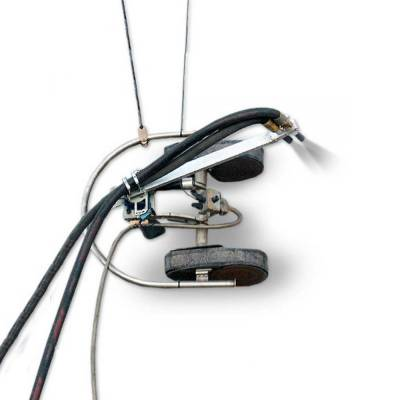
\includegraphics[width=8.4cm]{figs/cables/torbo}
	\caption{Robô TorboMate "Crawler", \cite{torbo}}
	\label{fig:cables:torbo}
\end{figure}

RIWEA é um robô puramente cabeado, no sentido em que ele não possui nenhum
outro tipo de forma de ajuste de posição além do sistema de cabos. É um
conceito de robô de estrutura aberta que faz uso de quatro cordas para se
deslocar verticamente \citep{jeon2012maintenance}. Seu maior diferencial reside
na capacidade de se adaptar a curvatura da pá mantendo sempre um ponto de apoio
sobre ela, sendo também menos suceptivel a vibrações \citep{riwea}.

\begin{figure}[!h]
	\centering
	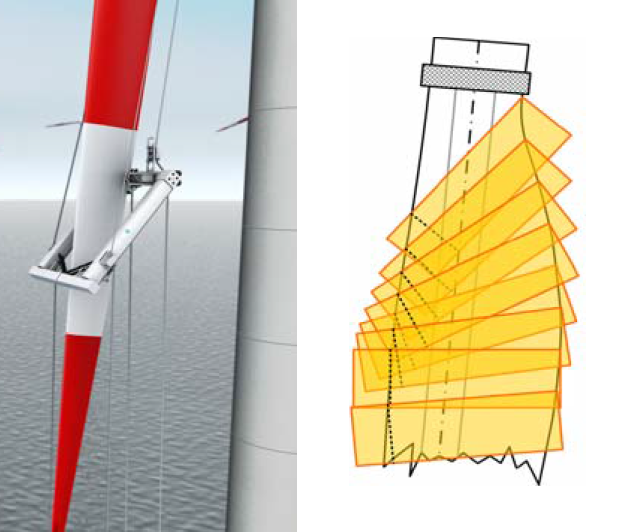
\includegraphics[width=8.4cm]{figs/cables/riwea}
	\caption{Robô RIWEA, sua cinemática adaptável ao formato da pá, \cite{riwea}}
	\label{fig:cables:riwea}
\end{figure}

Em geral, podemos sumarizar as caraterísticas do robôs cabeados segundo as
seguintes vantagens e desvantagens.

\textbf{Vantagens:}
\begin{itemize}
  \item Redução da carga sobre a fixação robô / maior capacidade de carga.
  \item Alcance do robô pelo cabeamento pode ser estendido a baixo custo.  
\end{itemize}

\textbf{Desvantagens:}
\begin{itemize}
  \item Complexidade do sistema de gestão do cabeamento.
  \item Necessidade de um ponto de apóio superior para fixação dos cabos.
\end{itemize}


